\chapter{System Architecture and Developed Mechanisms}

As the main proposed goal of this work is the implementation of a system that complies with the ALTO working group's devised protocol, this chapter exhibits the planned software specifications needed to implement the system as a whole.

Initial attention is given to the general architecture on the first section, with the goal of identifying key entities, their purpose, and how they interact among themselves. The following section will target the specification of ALTO resources, which can be considered the driving force behind the system, as they are what the client entities seek, and likewise what the ISPs wish to provide. The next section will focus on specifying the task of network intelligence provision to an appropriate ALTO server, in such a way that a common interface exists among all entities that are able to increase the server's knowledge of the network's physical topology. Specified the way that network information is provided, the next section details how a given actor, such as an ISP administrator, can manipulate such information before it is forwarded to the server - which includes the insertion of static ISP preferences or the abstraction of network entities as a means to dilute concrete topology details without forfeiting the usefulness the clients can retrieve from the processed resources. Finally, the task of inter-ISP ALTO server synchronization and communication is specified in the form of required protocol extensions and needed mechanisms that allows the increase of a single ALTO server's knowledge domain.

\subsection{System Architecture}

Figure \ref{fig:architecture-network} presents a high-level conceptual model of how the network information flows in a given ISP. Network data originates in the topology itself, and is gathered into a network intelligence aggregator by any given means, means as direct as importing a file that contains all the needed data, or as complex as a cluster of nodes that inspect the network for routing protocol packet messages and query nodes for physical properties and inject the resulting data into a central aggregator. Such intelligence is then parsed and uploaded to the ALTO server.

\textbf{NOTA: falta legendas, bolas brancas seriam nós físicos normais, bolas azuis seriam peers de uma aplicação P2P, triângulo azul seria um tracker, quadrado azul seria um cliente que precisa de escolher entre mirrors de dados, e poderia adicionar outro que precisa de escolher entre edge servers CDN. A ideia é mostrar que qualquer nó pode contactar o servidor ALTO para o seu propósito, e a agregação de dados ocorre na rede física toda.}

\begin{figure}[!h]
        \centering
        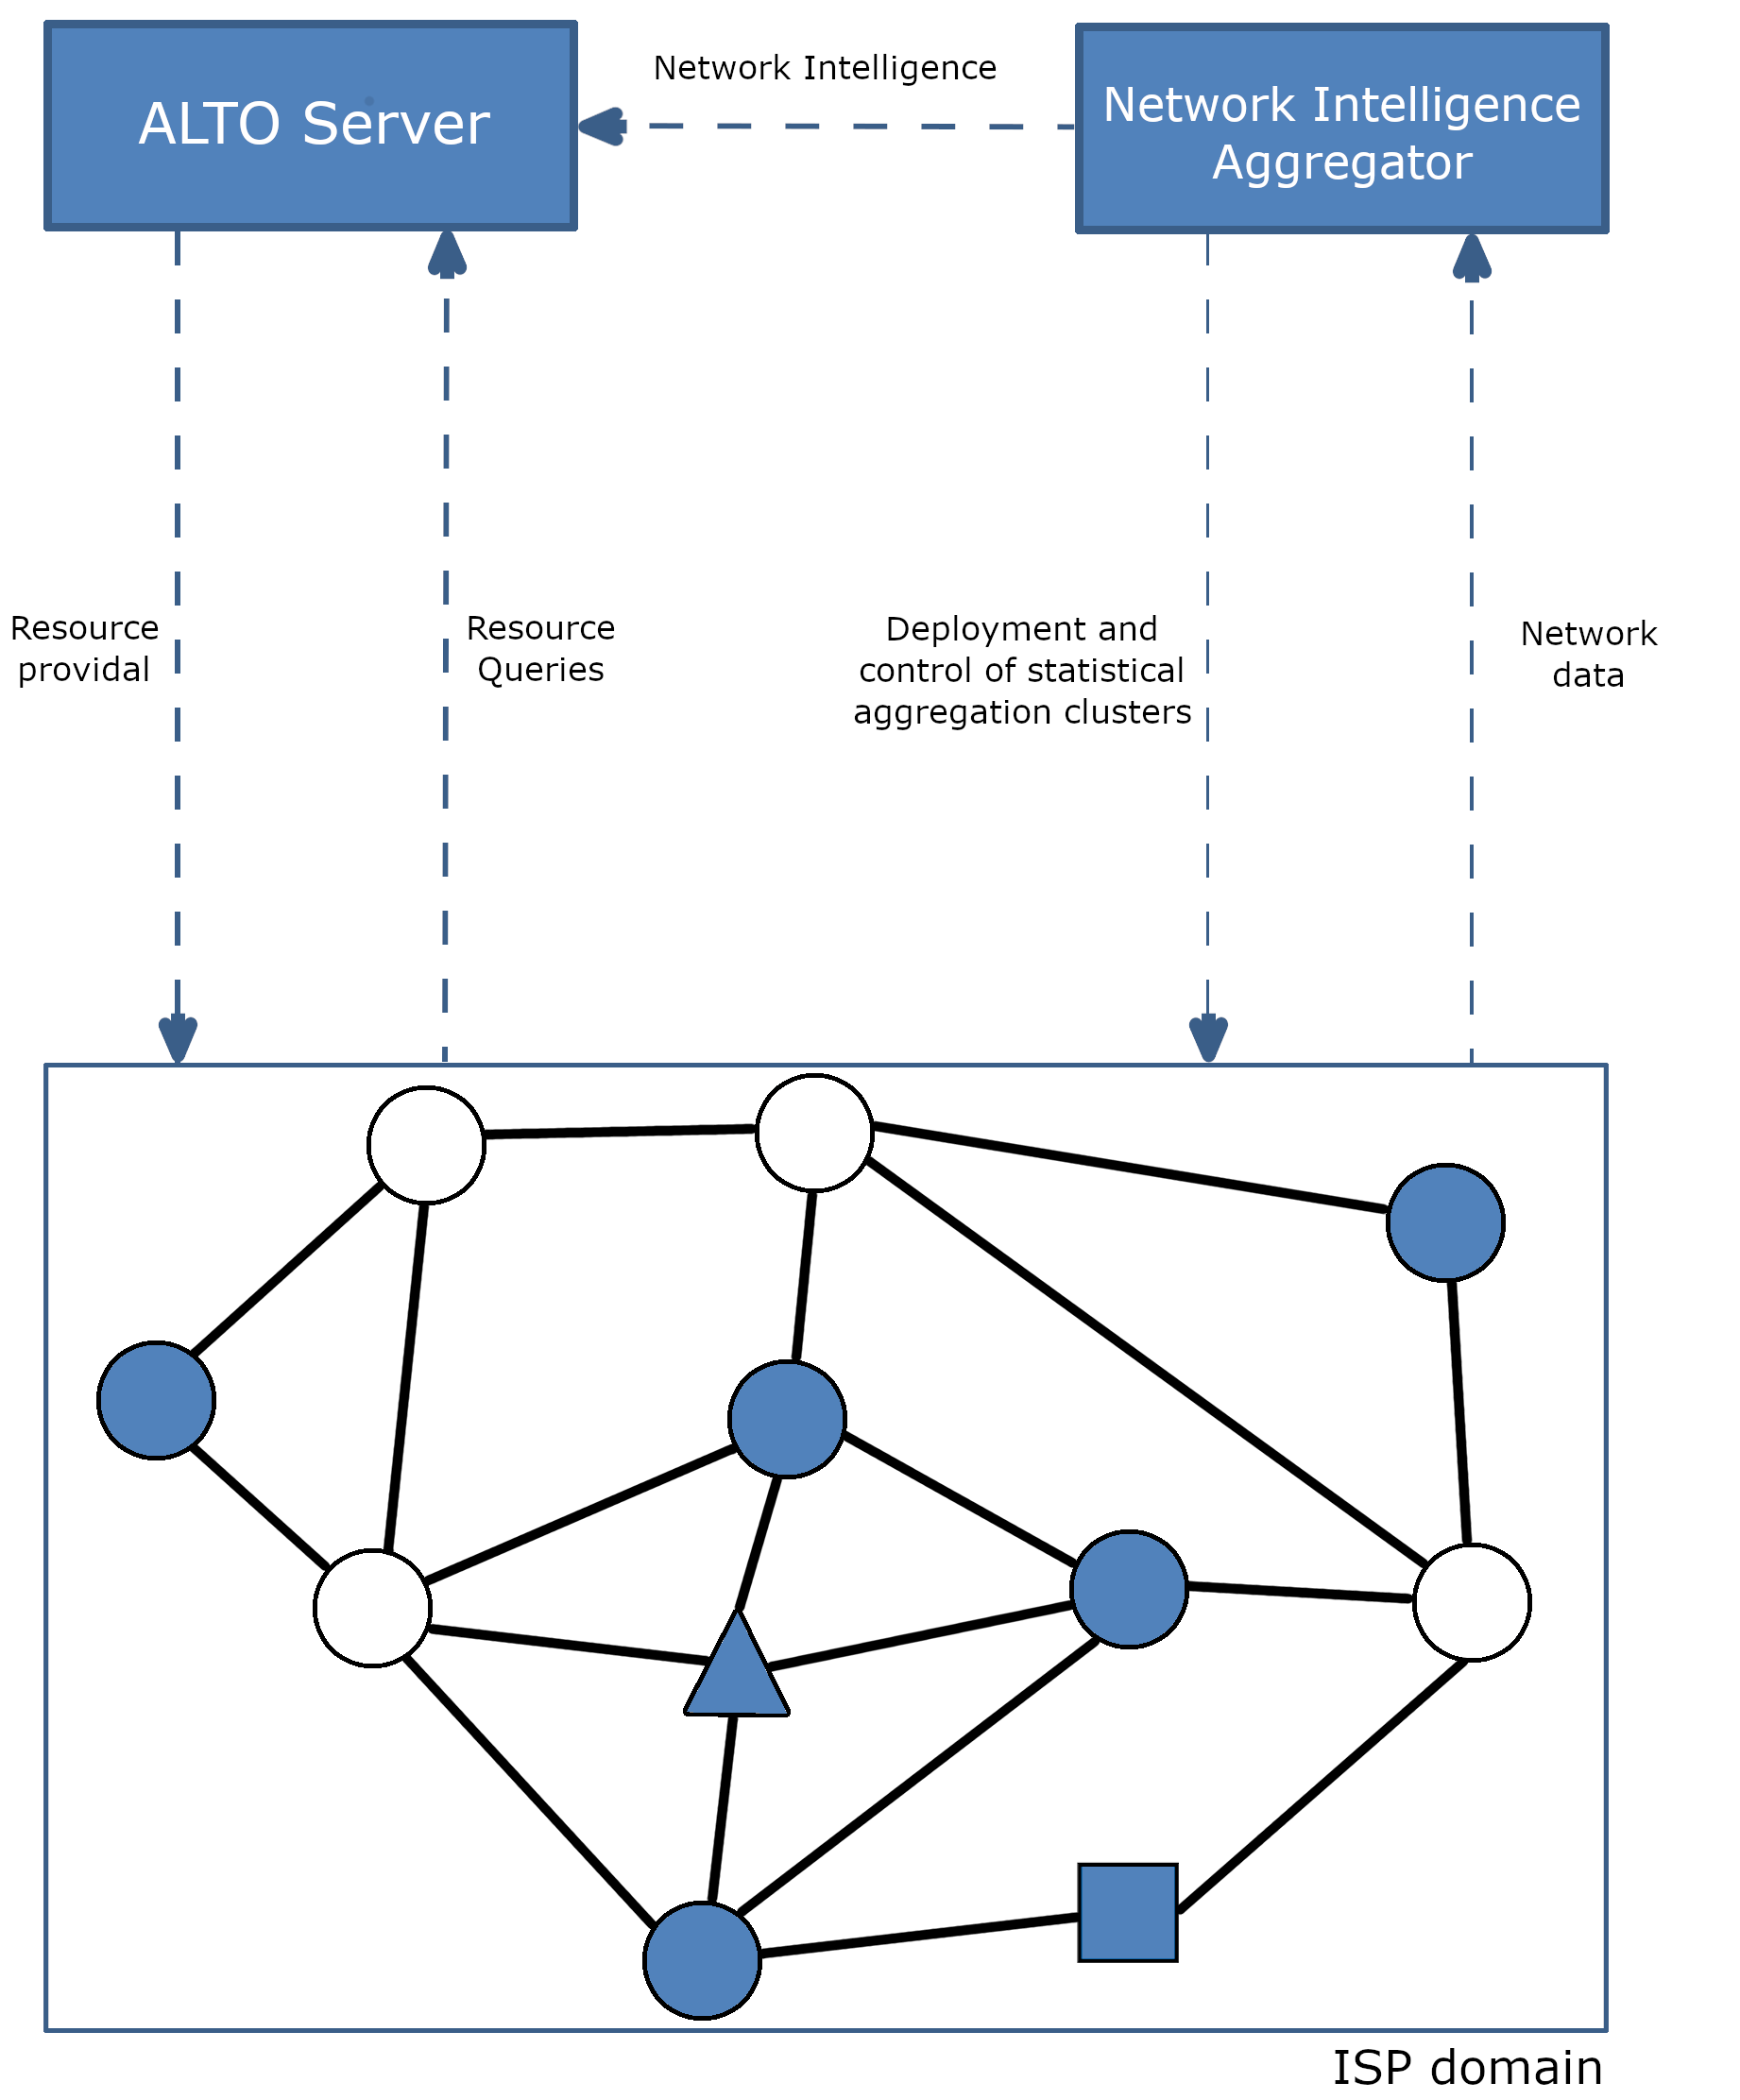
\includegraphics[scale=0.75]{img/architecture-network.png}
        \caption{Conceptual representation of the ALTO system of a given ISP}
        \label{fig:architecture-network}
\end{figure}

More formally, Figure \ref{fig:macro-architecture} presents the proposed system architecture. One can identify the ALTO interface as a key component of the system, as it allows to bridge three different application layers - the ALTO resource consumer, the ALTO resource provider, and the network intelligence aggregator, to be further specified in the following sections. The ALTO working group has extensively specified the ALTO protocol in regards to resource query, and the concrete implementation of this work will aim to fully comply to it. However, no resource provisioning protocol was, at time of writing, specified by the working group, nor was an interface been specified to allow network data to reach the ALTO server. With this in mind, this work specifies a protocol extension that enables a provisioning party to interact with an ALTO server with the intent to provide it with ALTO resources.

\begin{figure}[!h]
        \centering
        \includegraphics[scale=0.25]{architecture-macro.png}
        \caption{System architecture at a macro level}
        \label{fig:macro-architecture}
\end{figure}

\subsubsection{ALTO Resource Consumer}

An ALTO resource consumer is materialized in the architecture in the form of an ALTO client, which can be any entity who is able to interface with an ALTO server to query for ALTO resources. Whilst the ALTO working group was initially devised to help increase traffic localization via the sharing of network information, it now has an increased scope where an ideal client is any application which generates network traffic and would be able to optimize it with aid from an oracle entity with privileged network information. Thus, an ALTO client is fit to be implemented in P2P applications, and could be embedded in a P2P client itself to help with picking neighbouring and content providing nodes, or on a tracker that would accomplish the same goal on behalf of the querying peer. Likewise, nodes which are unable to optimally select between content which resides redundantly on many other nodes, such as CDN edge nodes or content mirrors, could also benefit from oracle guidance, and thus qualify as appropriate ALTO clients.

\subsubsection{ALTO Resource Provider}

An ALTO resource provider is materialized in the form of an ALTO server, an entity that possesses pre-processed network information in the form of ALTO resources. Its job is to store and manage such resources, and provide it to querying ALTO clients. Additionally, data validation and persistence are responsibilities that belong to the resource provider layer. Conceptually, the ALTO server is seen as a single entity, but considering the sensible information that could be stored within it and the influence it has on shaping netwokr traffic, it would not be uncommon for an ALTO server to have a knowledge domain correspondent to the ISP that owns it. Physically, though, the resource provider layer could consist of many interlinked ALTO providers with an increased coverage area of network knowledge. Means through which this could occur are further specified in section \ref{ssec:multi-alto}.

\subsubsection{Network Intelligence aggregation}

The network intelligence aggregation layer is the layer that enables the translation of raw topological information - such as the physical attributes of network devices and connections - and processed, query-eligible network knowledge. To do so, a very important entity, perhaps the heart of the system as a whole, is the network intelligence provider, which is responsible for retrieving network information and sending it, through a well defined network intelligence provisioning protocol, to a network intelligence aggregator. This latter entity is then responsible for providing the ALTO resource provider layer with valid information after the raw topological data has been processed - this includes the calculation of optimal paths, the abstraction of network entities, or the injection of static ISP preferences.


\subsection{ALTO resources}
\label{ssec:alto-resources}

ALTO resources are pieces of network information which are provided by an ALTO server and consumed by ALTO clients that ideally would use such information to aid their applicational decisions. All ALTO resources must have the following:

\begin{itemize}
        \item \textbf{Meta information}: data which regards to the resource's profile, that enable the client's ability to interpret and cross-reference the network data within. Following suit to the defined protocol, meta information contains the resource's name, version and, if applicable, resource dependencies and cost details - its mode, metric name, and description.
        \item \textbf{Network information}: data structures that give a characterization of the ALTO Server's vision of a network. Concretely, these can map network properties to a node (such the connection types of their interfaces, or their geographical location), they can aggregate many network addresses to a single identifier, or they can map properties to a node link or end-to-end path (such as link or cumulative routing costs, respectively).
\end{itemize}{}

\todo{Speak of Information Resource Directories}

Further formal specification is not made as it has been extensively done in the ALTO protocol \cite{alto-protocol}. Figure \ref{fig:alto-resources} summarizes the alto resource specification and lists the concrete resource types they can be materialized into, each with their well defined structure that is expected to be known by entities that interact with the ALTO interface.

\todo{Add network map to image}
\begin{figure}[!h]
        \centering
        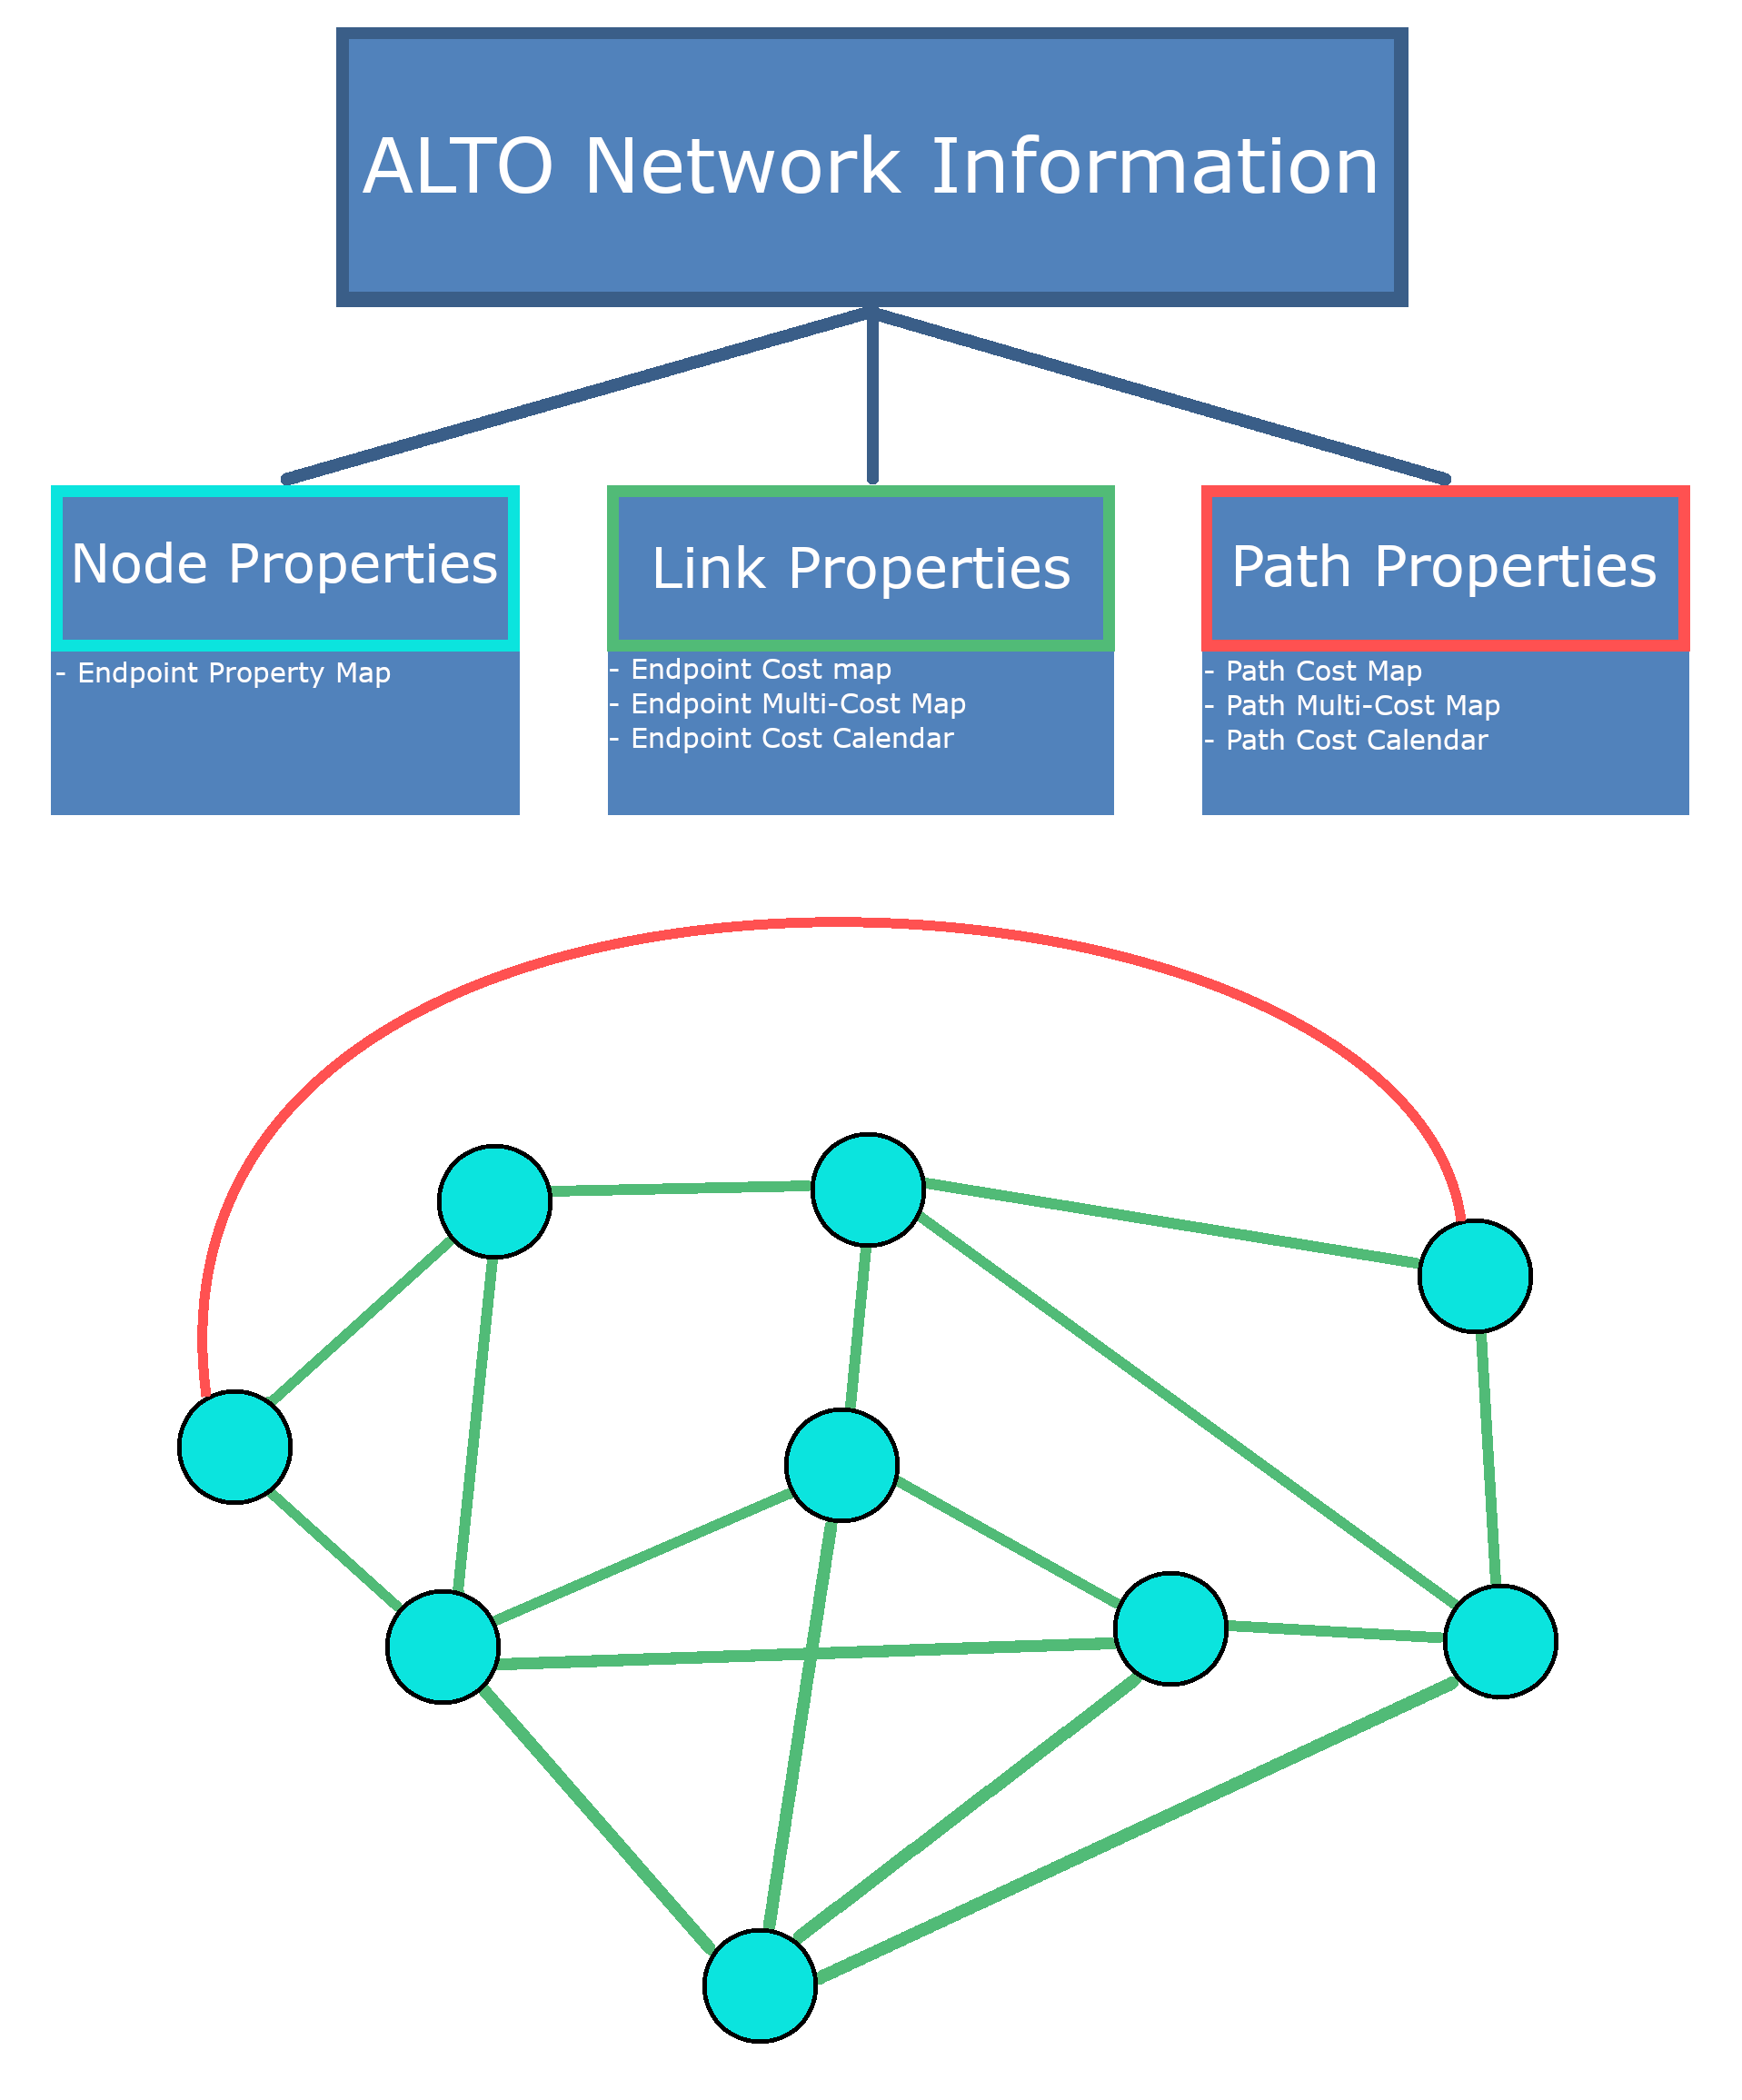
\includegraphics[scale=0.80]{img/architecture-resources.png}
        \caption{Schematization of the pondered ALTO resources}
        \label{fig:alto-resources}
\end{figure}

\subsection{Network intelligence provision}

\subsection{Network intelligence preprocessing}

\subsection{Multi ALTO server communication}
\label{ssec:multi-alto}

